\documentclass[12pt]{article}
\usepackage[utf8]{inputenc}
\usepackage[catalan]{babel}
\usepackage{amsmath, amssymb, amsfonts}
\usepackage{geometry}
\usepackage{fancyhdr}
\usepackage{tikz}
\usetikzlibrary{matrix, calc, positioning, arrows.meta}
\usepackage{tcolorbox}
\usepackage[colorlinks=true, linkcolor=blue]{hyperref}
\usepackage{float}
\usepackage{enumitem}

\setlength{\headheight}{15pt}

% Definicions de geometria
\geometry{a4paper, left=2cm, right=2cm, top=2.5cm, bottom=2.5cm}

% Configuració de l'encapçalament i peu de pàgina
\pagestyle{fancy}
\fancyhf{}
\fancyhead[L]{Matemàtiques 2n Batxillerat}
\fancyhead[R]{Vectors a l'espai}
\fancyfoot[L]{\href{mailto:orodri11@xtec.cat}{orodri11@xtec.cat}}
\fancyfoot[R]{\thepage}

% Estils per a quadres
\newtcolorbox{concept}[1][]{colback=blue!5!white, colframe=blue!75!black, fonttitle=\bfseries, title=Concepte, #1}
\newtcolorbox{exemple}[1][]{colback=green!5!white, colframe=green!75!black, fonttitle=\bfseries, title=Exemple, #1}
\newtcolorbox{exercici}[1][]{colback=yellow!5!white, colframe=yellow!75!black, fonttitle=\bfseries, title=Exercici, #1}

\begin{document}

% Portada
\begin{titlepage}
    \centering
    {\Huge \textbf{Vectors a l'espai \\ 2n Batxillerat} \par}
    \vspace{1cm}
    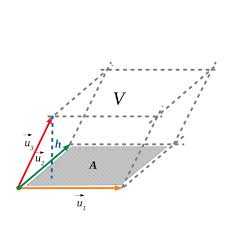
\includegraphics[width=0.5\textwidth]{baixa.png}
    \vspace{1cm}
    \tableofcontents
\end{titlepage}

\newpage

\section{Vectors a l'espai}

\subsection{Localització de punts a l'espai}

\begin{concept}
Per determinar la posició d'un punt a l'espai, cal definir un sistema de referència. 
El més habitual està format per tres rectes perpendiculars entre elles que es tallen en un punt $O$, anomenat origen de coordenades[reference:3]. 

Aquestes tres rectes s'anomenen eixos de coordenades i es designen per $X$, $Y$ i $Z$.

Fixada una unitat de longitud:
\begin{itemize}
    \item La posició de qualsevol punt $P$ de l'espai determina una única terna ordenada $(x, y, z)$ de nombres reals.
    \item Recíprocament, cada terna ordenada de nombres reals $(x, y, z)$ correspon a un únic punt $P$ de l'espai.
\end{itemize}

\begin{center}
\begin{tikzpicture}[scale=1.5]
    % Eixos
    \draw[->] (0,0,0) -- (2,0,0) node[anchor=north east] {$X$};
    \draw[->] (0,0,0) -- (0,2,0) node[anchor=north west] {$Y$};
    \draw[->] (0,0,0) -- (0,0,2) node[anchor=south] {$Z$};

    % Punt P
    \draw[fill=red] (1,1,1) circle (1pt) node[anchor=south east] {$P(x, y, z)$};

    % Guies
    \draw[dashed] (1,1,1) -- (1,1,0);
    \draw[dashed] (1,1,0) -- (1,0,0);
    \draw[dashed] (1,1,0) -- (0,1,0);
\end{tikzpicture}
\end{center}
\end{concept}

\begin{exemple}
Considerem el punt $P(4, 0, -3)$. Les seves coordenades indiquen:
\begin{itemize}
    \item $x = 4$: Posició en l'eix $X$.
    \item $y = 0$: El punt està sobre el pla $XZ$.
    \item $z = -3$: Es troba a una distància de $3$ unitats per sota del pla $XY$.
\end{itemize}
\end{exemple}

\begin{exercici}
Indica en cada cas com identificaries, a partir de les seves coordenades:
\begin{enumerate}
    \item Un punt de l'eix $X$.
    \item Un punt de l'eix $Y$.
    \item Un punt de l'eix $Z$.
    \item Un punt del pla $XY$.
    \item Un punt del pla $YZ$.
    \item Un punt del pla $XZ$.
\end{enumerate}
\end{exercici}

\subsection{Vectors a l'espai}

\begin{concept}
Siguin dos punts $A(a_1, a_2, a_3)$ i $B(b_1, b_2, b_3)$ a l'espai[reference:4]. Els components del vector fix $\overrightarrow{AB}$, amb origen al punt $A$ i extrem al punt $B$, s'obtenen restant a les coordenades de l'extrem les coordenades de l'origen[reference:5]:
\[
\overrightarrow{AB} = (b_1 - a_1, b_2 - a_2, b_3 - a_3)
\]

Es diu que dos vectors $\overrightarrow{AB}$ i $\overrightarrow{CD}$ són equipol·lents si tenen la mateixa longitud, direcció i sentit[reference:6].
\end{concept}

\begin{exemple}
Donats els punts $A(3, -1, 5)$ i $B(6, -2, 3)$, trobem els components del vector $\overrightarrow{AB}$:
\[
\overrightarrow{AB} = (6 - 3, -2 - (-1), 3 - 5) = (3, -1, -2)
\]
\end{exemple}

\begin{exercici}
Donats els punts:
\begin{enumerate}
    \item $A(3, -1, 5)$ i $B(6, -2, 3)$, troba els components del vector $\overrightarrow{AB}$.
    \item Si $\overrightarrow{CD} = (3, -6, 0)$ i $C(-1, 4, 3)$, troba les coordenades del punt $D$.
\end{enumerate}
\end{exercici}

\subsection{Vector posició i mòdul d'un vector}

\begin{concept}
El conjunt de tots els vectors fixos equipol·lents entre ells s'anomena vector lliure[reference:7]. Entre aquests vectors, n'hi ha un amb origen a $O$ i extrem a $P$, anomenat vector posició $\overrightarrow{OP}$. Els seus components són les coordenades de $P$[reference:8].

El mòdul d'un vector $\vec{v} = (v_1, v_2, v_3)$ es defineix com[reference:9]:
\[
|\vec{v}| = \sqrt{v_1^2 + v_2^2 + v_3^2}
\]
\end{concept}

\begin{exemple}
Sigui el vector $\vec{v} = (3, -4, 0)$. El seu mòdul és:
\[
|\vec{v}| = \sqrt{3^2 + (-4)^2 + 0^2} = \sqrt{9 + 16} = 5
\]
\end{exemple}

\begin{exercici}
Troba el mòdul dels vectors següents:
\begin{enumerate}
    \item $\vec{u} = (2, -2, 1)$
    \item $\vec{w} = (0, 0, 0)$
\end{enumerate}
\end{exercici}

\section{Operacions amb vectors}

\subsection{Suma de vectors}

\begin{concept}
La suma de dos vectors de l'espai, $\vec{a} = (a_1, a_2, a_3)$ i $\vec{b} = (b_1, b_2, b_3)$, es calcula component a component[reference:10]:
\[
\vec{a} + \vec{b} = (a_1 + b_1, a_2 + b_2, a_3 + b_3).
\]
Gràficament, el vector suma és el vector que uneix l'origen de $\vec{a}$ amb l'extrem de $\vec{b}$, seguint la regla del paral·lelogram[reference:11].
\end{concept}

\begin{figure}[htbp]
    \centering
    \begin{tikzpicture}
        % Vectors
        \draw[->, thick] (0,0) -- (2,1) node[midway, above] {$\vec{a}$};
        \draw[->, thick] (0,0) -- (1,3) node[midway, left] {$\vec{b}$};
        \draw[->, dashed] (2,1) -- (3,4);
        \draw[->, dashed] (1,3) -- (3,4);
        \draw[->, thick, red] (0,0) -- (3,4) node[midway, right] {$\vec{a} + \vec{b}$};
    \end{tikzpicture}
    \caption{Representació gràfica de la suma de vectors seguint la regla del paral·lelogram.}
    \label{fig:suma_vectors}
\end{figure}

\begin{exemple}
Dona els components del vector suma de $\vec{a} = (2, -1, 3)$ i $\vec{b} = (1, 4, -2)$.
\[
\vec{a} + \vec{b} = (2+1, -1+4, 3+(-2)) = (3, 3, 1).
\]
\end{exemple}

\begin{exercici}
Donats els vectors $\vec{a} = (1, 3, 2)$, $\vec{b} = (3, 1, -1)$ i $\vec{c} = (0, 0, 3)$, troba els components dels vectors:
\begin{enumerate}[label=\alph*)]
    \item $2\vec{a} + 3\vec{b} - \vec{c}$
    \item $\vec{a} - 3(2\vec{b} + \vec{c})$
\end{enumerate}
\end{exercici}

\subsection{Subtracció de vectors}

\begin{concept}
Com que restar un vector és el mateix que sumar l'oposat[reference:12], la subtracció de vectors queda definida de la següent manera:
\[
\vec{a} - \vec{b} = \vec{a} + (-\vec{b}) = (a_1 - b_1, a_2 - b_2, a_3 - b_3)
\]
\end{concept}

\subsection{Propietats de la suma de vectors}
\begin{concept}
\begin{itemize}
    \item \textbf{Commutativa}: 
    \[
    \vec{a} + \vec{b} = \vec{b} + \vec{a}
    \]
    \item \textbf{Associativa}[reference:13]:
    \[
    \vec{a} + (\vec{b} + \vec{c}) = (\vec{a} + \vec{b}) + \vec{c}
    \]
    \item \textbf{Existència d'element neutre}[reference:14]: El vector nul $0 = (0,0,0)$ és l'element neutre per a la suma de vectors:
    \[
    \vec{a} + \vec{0} = \vec{a}
    \]
    \item \textbf{Existència d'element simètric}[reference:15]: Cada vector $\vec{a}$ té un vector simètric, que és el seu oposat $-\vec{a}$, tal que:
    \[
    \vec{a} + (-\vec{a}) = \vec{0}
    \]
\end{itemize}
\end{concept}

\subsection{Multiplicació d'un vector per un nombre real}

\begin{concept}
Sigui $\vec{a} = (a_1, a_2, a_3)$ i $k \in \mathbb{R}$. El producte de $k$ per $\vec{a}$ és el vector que té per components $(ka_1, ka_2, ka_3)$[reference:16]:
\[
k \cdot \vec{a} = k \cdot (a_1, a_2, a_3) = (ka_1, ka_2, ka_3)
\]

Si $k \neq 0$, aleshores els vectors $\vec{a}$ i $k \cdot \vec{a}$ tenen la mateixa direcció. Si $k > 0$, també tenen el mateix sentit i si $k < 0$, tenen sentits oposats[reference:17]. Pel que fa al mòdul[reference:18]:
\[
|k \cdot \vec{a}| = |k| \cdot |\vec{a}|
\]
\end{concept}

\subsection{Propietats de la multiplicació d'un vector per un nombre real}

\begin{concept}
\begin{itemize}
    \item \textbf{Distributiva respecte a la suma de vectors}:
    \[
    k \cdot (\vec{a} + \vec{b}) = k \cdot \vec{a} + k \cdot \vec{b}
    \]
    \item \textbf{Distributiva respecte a la suma de nombres reals}:
    \[
    (k + h) \cdot \vec{a} = k \cdot \vec{a} + h \cdot \vec{a}
    \]
    \item \textbf{Associativa}:
    \[
    (k \cdot h) \cdot \vec{a} = k \cdot (h \cdot \vec{a})
    \]
    \item \textbf{Existència d'element neutre}:
    \[
    1 \cdot \vec{a} = \vec{a}
    \]
\end{itemize}
\end{concept}

\subsection{Vector unitari}

\begin{concept}
Un vector es diu unitari si el seu mòdul és 1[reference:19]. Qualsevol vector $\vec{v}$ no nul té associat un vector unitari $\vec{u}$ amb la mateixa direcció i sentit[reference:20]. Es calcula multiplicant el vector $\vec{v}$ per l'invers del seu mòdul:
\[
\vec{u} = \frac{1}{|\vec{v}|} \vec{v}
\]
\end{concept}

\subsection{Combinació lineal, dependència i bases}

\subsubsection{Combinació lineal de vectors}

\begin{concept}
Donats un conjunt de vectors $\vec{v}_1, \vec{v}_2, \dots, \vec{v}_n$ i un conjunt de nombres reals $a_1, a_2, \dots, a_n$, s'anomena \textbf{combinació lineal} dels vectors al vector:
\[
\vec{w} = a_1\vec{v}_1 + a_2\vec{v}_2 + \dots + a_n\vec{v}_n
\]
Els nombres $a_i$ s'anomenen \textbf{coeficients} de la combinació lineal.
\end{concept}

\begin{exemple}
Donats $\vec{a} = (1, 2, 0)$ i $\vec{b} = (0, -1, 3)$, una combinació lineal és:
\[
2\vec{a} - 3\vec{b} = 2(1, 2, 0) - 3(0, -1, 3) = (2, 4, 0) + (0, 3, -9) = (2, 7, -9)
\]
\end{exemple}

\begin{exercici}
Escriu el vector $\vec{w} = (5, -1, 4)$ com a combinació lineal de $\vec{u} = (1, 1, 1)$, $\vec{v} = (1, -1, 0)$ i $\vec{t} = (1, 0, -1)$.
\end{exercici}

\subsubsection{Dependència i independència lineal}

\begin{concept}
Un conjunt de vectors és \textbf{linealment dependent} si algun d'ells es pot expressar com a combinació lineal dels altres. En cas contrari, són \textbf{linealment independents}.

Per a vectors a l'espai ($\mathbb{R}^3$):
\begin{itemize}
    \item \textbf{Dos vectors} són linealment dependents si són proporcionals (és a dir, un és múltiple escalar de l'altre).
    \item \textbf{Tres vectors} $\vec{u}, \vec{v}, \vec{w}$ són linealment independents si el determinant de la matriu que formen és diferent de zero.
\end{itemize}
\end{concept}

\begin{exemple}
Els vectors $\vec{a} = (1, 2, 3)$ i $\vec{b} = (2, 4, 6)$ són dependents perquè $\vec{b} = 2\vec{a}$.

Els vectors $\vec{a} = (1, 0, 0)$, $\vec{b} = (0, 1, 0)$ i $\vec{c} = (0, 0, 1)$ són independents perquè cap es pot escriure com a combinació dels altres (el determinant de la matriu identitat és 1).
\end{exemple}

\begin{exercici}
Determina si els vectors $\vec{u} = (1, 1, 0)$, $\vec{v} = (0, 1, 1)$ i $\vec{w} = (1, 0, 1)$ són linealment independents.
\end{exercici}

\subsubsection{Bases d'un espai vectorial}

\begin{concept}
Una \textbf{base} d'un espai vectorial és un conjunt de vectors que compleix dues condicions:
\begin{enumerate}
    \item Són \textbf{linealment independents}.
    \item \textbf{Generen} tot l'espai (és a dir, qualsevol vector de l'espai es pot escriure com a combinació lineal dels vectors de la base).
\end{enumerate}

A l'espai tridimensional ($\mathbb{R}^3$), una base està formada per 3 vectors linealment independents. La base més habitual és la \textbf{base canònica}[reference:21]:
\[
\vec{i} = (1, 0, 0), \quad \vec{j} = (0, 1, 0), \quad \vec{k} = (0, 0, 1)
\]
\end{concept}

\begin{exemple}
Qualsevol vector $\vec{v} = (x, y, z)$ es pot escriure com a combinació lineal de la base canònica:
\[
\vec{v} = x\vec{i} + y\vec{j} + z\vec{k}
\]
Per exemple, $\vec{v} = (3, -2, 5) = 3\vec{i} - 2\vec{j} + 5\vec{k}$.
\end{exemple}

\begin{exercici}
Comprova que els vectors $\vec{a} = (1, 1, 0)$, $\vec{b} = (1, -1, 0)$ i $\vec{c} = (0, 0, 1)$ formen una base de $\mathbb{R}^3$.
\end{exercici}

\section{La recta a l'espai}

\subsection{Equacions de la recta}

\begin{concept}
Per determinar una recta a l'espai ens fa falta un punt que hi pertanyi i un vector director, que és aquell que té la mateixa direcció que la recta[reference:22].

Donat un punt qualsevol $P=(a,b,c)$ d'una recta $r$, i un vector director d'aquesta recta, $\vec{u}=(u_1,u_2,u_3)$, podem afirmar que un punt $X=(x,y,z)$ pertany a la recta $r$ si el podem obtenir a partir de sumar al punt $P$ un determinat nombre de vegades ($\lambda$, $\lambda\in\mathbb{R}$) la direcció del vector $\vec{u}$[reference:23]:

\[
\boxed{(x,y,z)=(a,b,c)+\lambda(u_1,u_2,u_3)}
\]

Aquesta és l'equació \textbf{vectorial} de la recta[reference:24].

Si igualem component a component l'equació anterior obtenim les \textbf{equacions paramètriques} de la recta[reference:25]:
\[
\boxed{
\begin{cases}
x = a + \lambda u_1 \\
y = b + \lambda u_2 \\
z = c + \lambda u_3
\end{cases}
}
\]

Si aïllem la $\lambda$ de les equacions anteriors, obtenim l'equació \textbf{contínua} de la recta[reference:26]:
\[
\boxed{\frac{x-a}{u_1} = \frac{y-b}{u_2} = \frac{z-c}{u_3}}
\]

Finalment, si agrupem les equacions anteriors dues a dues, obtindrem l'equació \textbf{implícita o cartesiana} de la recta[reference:27]:
\[
\boxed{
\begin{cases}
Ax + By + Cz + D = 0 \\
A'x + B'y + C'z + D' = 0
\end{cases}
}
\]
\end{concept}

\begin{exemple}
Dóna l'equació de la recta que passa pel punt $P=(2,1,0)$ i és paral·lela a la recta d'equació paramètrica[reference:28]:
\[
\begin{cases}
x = 3 + \lambda \\
y = 2 + 2\lambda \\
z = 3 - \lambda
\end{cases}
\]

Si és paral·lela a aquesta recta, tindrà el mateix vector director: $\vec{u}=(1,2,-1)$[reference:29]. Si tenim el punt i el vector, podem donar aquesta recta utilitzant l'equació contínua[reference:30]:
\[
\frac{x-2}{1} = \frac{y-1}{2} = \frac{z-0}{-1}
\]
\end{exemple}

\subsection{Equacions dels eixos de coordenades}

\begin{concept}
Els eixos de coordenades ($x$, $y$ i $z$) tenen vectors directors (base canònica) $\vec{i}=(1,0,0)$, $\vec{j}=(0,1,0)$ i $\vec{k}=(0,0,1)$ respectivament[reference:31].

Si prenem les equacions paramètriques de la recta i aquests vectors obtenim[reference:32]:

\begin{center}
\begin{tabular}{|c|c|c|}
\hline
\textbf{Eix $x$} & \textbf{Eix $y$} & \textbf{Eix $z$} \\
\hline
$\begin{cases} x = \lambda \\ y = 0 \\ z = 0 \end{cases}$ &
$\begin{cases} x = 0 \\ y = \lambda \\ z = 0 \end{cases}$ &
$\begin{cases} x = 0 \\ y = 0 \\ z = \lambda \end{cases}$ \\
\hline
\end{tabular}
\end{center}
\end{concept}

\section{El pla a l'espai}

\subsection{Equacions del pla}

\begin{concept}
Si per definir una recta necessitàvem una direcció (vector) i un punt de la recta, per a definir un pla necessitarem 3 elements: un punt $P=(a,b,c)$ del pla, i un parell de vectors $\vec{u}=(u_1,u_2,u_3)$ i $\vec{v}=(v_1,v_2,v_3)$ \textbf{linealment independents} que es trobin dins del pla[reference:33].

A partir d'aquí, qualsevol punt del pla $X=(x,y,z)$ es pot escriure com:
\[
\boxed{(x,y,z)=(a,b,c)+\lambda(u_1,u_2,u_3)+\mu(v_1,v_2,v_3)}
\]
Aquesta és l'equació \textbf{vectorial} del pla.

Si igualem component a component obtenim les \textbf{equacions paramètriques} del pla:
\[
\boxed{
\begin{cases}
x = a + \lambda u_1 + \mu v_1 \\
y = b + \lambda u_2 + \mu v_2 \\
z = c + \lambda u_3 + \mu v_3
\end{cases}
}
\]

Finalment, l'equació \textbf{general o implícita} del pla és de la forma:
\[
\boxed{Ax + By + Cz + D = 0}
\]
on el vector $\vec{n} = (A, B, C)$ és un vector \textbf{normal} al pla.
\end{concept}

\begin{exemple}
Troba l'equació del pla que passa pels punts $A(1,0,0)$, $B(0,1,0)$ i $C(0,0,1)$.

Prenem com a punt del pla $A(1,0,0)$ i com a vectors directors:
\[
\vec{u} = \overrightarrow{AB} = (-1,1,0), \quad \vec{v} = \overrightarrow{AC} = (-1,0,1)
\]
L'equació vectorial és:
\[
(x,y,z) = (1,0,0) + \lambda(-1,1,0) + \mu(-1,0,1)
\]
Les equacions paramètriques:
\[
\begin{cases}
x = 1 - \lambda - \mu \\
y = \lambda \\
z = \mu
\end{cases}
\]
Si substituïm $\lambda = y$ i $\mu = z$ a la primera equació, obtenim l'equació implícita:
\[
x = 1 - y - z \quad \Rightarrow \quad x + y + z = 1
\]
\end{exemple}

\begin{exercici}
Troba l'equació del pla que passa pel punt $P(2,1,-1)$ i té com a vectors directors $\vec{u}=(1,0,2)$ i $\vec{v}=(0,1,-1)$.
\end{exercici}

\section{Problemes mètrics}

\subsection{Distància entre dos punts}

\begin{concept}
La distància entre 2 punts $A(a_1,a_2,a_3)$ i $B(b_1,b_2,b_3)$ a $\mathbb{R}^3$ és el mòdul del vector format per aquests punts[reference:34]:
\[
\boxed{d(A,B) = |\overrightarrow{AB}| = \sqrt{(b_1-a_1)^2 + (b_2-a_2)^2 + (b_3-a_3)^2}}
\]
\end{concept}

\subsection{Distància d'un punt a una recta}

\begin{concept}
Donat un punt $P(a,b,c)$ i una recta $r$ qualsevol, la distància d'aquest punt a la recta s'obté calculant la projecció ortogonal del punt $P$ sobre la recta $r$, el punt $P'$[reference:35]. La distància serà el mòdul del vector $\overrightarrow{P'P}$[reference:36].
\end{concept}

\begin{exemple}
Troba la distància del punt $P(5,6,1)$ a la recta[reference:37]:
\[
r: \frac{x}{1} = \frac{y-1}{1} = \frac{z+1}{4}
\]

Expressem la recta amb l'equació paramètrica[reference:38]:
\[
r:
\begin{cases}
x = \lambda \\
y = 1 + \lambda \\
z = -1 + 4\lambda
\end{cases}
\]
Per tant, qualsevol punt de la recta $r$, i $P'$ en particular, tindrà la forma[reference:39]:
\[
P' = (\lambda, 1+\lambda, -1+4\lambda)
\]

Si calculem ara la distància entre $P$ i $P'$ a través del mòdul del vector $\overrightarrow{P'P}$, tenim que[reference:40]:
\[
\overrightarrow{P'P} = (5-\lambda, 6-(1+\lambda), 1-(-1+4\lambda)) = (5-\lambda, 5-\lambda, 2-4\lambda)
\]

Alhora, aquest vector és perpendicular al vector director de la recta, $\vec{v}=(1,1,4)$. Per tant, el seu producte escalar serà zero[reference:41]:
\[
\vec{v} \cdot \overrightarrow{P'P} = 1(5-\lambda) + 1(5-\lambda) + 4(2-4\lambda) = 0
\]
\[
5-\lambda + 5-\lambda + 8 - 16\lambda = 0 \quad \Rightarrow \quad 18 - 18\lambda = 0 \quad \Rightarrow \quad \lambda = 1
\]

Per tant, la projecció de $P$ sobre la recta $r$ és[reference:42]:
\[
P' = (1, 2, 3)
\]
i la distància del punt a la recta és[reference:43]:
\[
d(P,r) = |\overrightarrow{P'P}| = \sqrt{(5-1)^2 + (6-2)^2 + (1-3)^2} = \sqrt{16 + 16 + 4} = \sqrt{36} = 6
\]
\end{exemple}

\subsection{Distància entre dues rectes}

\begin{concept}
La distància entre dues rectes és la longitud del segment perpendicular comú a totes dues. Per calcular-la, es pot trobar el pla que conté una de les rectes i és paral·lel a l'altra, i després calcular la distància de qualsevol punt de l'altra recta a aquest pla.
\end{concept}

\subsection{Distància d'un punt a un pla}

\begin{concept}
Donat un punt $P(x_0, y_0, z_0)$ i un pla $\pi: Ax + By + Cz + D = 0$, la distància del punt al pla es calcula amb la fórmula:
\[
\boxed{d(P,\pi) = \frac{|Ax_0 + By_0 + Cz_0 + D|}{\sqrt{A^2 + B^2 + C^2}}}
\]
\end{concept}

\subsection{Angle entre dues rectes}

\begin{concept}
L'angle entre dues rectes és l'angle que formen els seus vectors directors. Si les rectes tenen vectors directors $\vec{u}$ i $\vec{v}$, l'angle $\alpha$ ve donat per:
\[
\cos \alpha = \frac{|\vec{u} \cdot \vec{v}|}{|\vec{u}| \cdot |\vec{v}|}
\]
\end{concept}

\subsection{Angle entre recta i pla}

\begin{concept}
L'angle entre una recta i un pla és l'angle que forma la recta amb la seva projecció ortogonal sobre el pla. Si la recta té vector director $\vec{u}$ i el pla té vector normal $\vec{n}$, l'angle $\alpha$ ve donat per:
\[
\sin \alpha = \frac{|\vec{u} \cdot \vec{n}|}{|\vec{u}| \cdot |\vec{n}|}
\]
\end{concept}

\subsection{Angle entre dos plans}

\begin{concept}
L'angle entre dos plans és l'angle que formen els seus vectors normals. Si els plans tenen vectors normals $\vec{n}_1$ i $\vec{n}_2$, l'angle $\alpha$ ve donat per:
\[
\cos \alpha = \frac{|\vec{n}_1 \cdot \vec{n}_2|}{|\vec{n}_1| \cdot |\vec{n}_2|}
\]
\end{concept}

\section{Exercicis finals}

\subsection{Vectors}

\begin{exercici}
Donats els vectors $\vec{u} = (2, -1, 3)$ i $\vec{v} = (1, 4, -2)$:
\begin{enumerate}[label=\alph*)]
    \item Calcula $\vec{u} + \vec{v}$ i $\vec{u} - \vec{v}$.
    \item Troba el mòdul de $\vec{u}$ i de $\vec{v}$.
    \item Determina si $\vec{u}$ i $\vec{v}$ són linealment dependents.
\end{enumerate}
\end{exercici}

\begin{exercici}
Donats els vectors $\vec{a} = (1, 2, 3)$, $\vec{b} = (4, 5, 6)$ i $\vec{c} = (7, 8, 9)$:
\begin{enumerate}[label=\alph*)]
    \item Comprova si són linealment dependents.
    \item Si és possible, expressa $\vec{c}$ com a combinació lineal de $\vec{a}$ i $\vec{b}$.
\end{enumerate}
\end{exercici}

\begin{exercici}
Donats els vectors $\vec{p} = (1, 0, -1)$, $\vec{q} = (0, 1, 0)$ i $\vec{r} = (1, 1, 1)$:
\begin{enumerate}[label=\alph*)]
    \item Demostra que formen una base de $\mathbb{R}^3$.
    \item Troba les coordenades del vector $\vec{w} = (2, -1, 3)$ en aquesta base.
\end{enumerate}
\end{exercici}

\subsection{Rectes i plans}

\begin{exercici}
Troba les equacions vectorial, paramètrica, contínua i implícita de la recta que passa pel punt $A(1,-2,3)$ i té vector director $\vec{u}=(2,-1,4)$.
\end{exercici}

\begin{exercici}
Troba l'equació del pla que passa pel punt $P(2,0,-1)$ i conté els vectors $\vec{u}=(1,2,3)$ i $\vec{v}=(0,-1,2)$.
\end{exercici}

\begin{exercici}
Troba l'equació del pla que passa pels punts $A(1,0,0)$, $B(0,2,0)$ i $C(0,0,3)$.
\end{exercici}

\subsection{Problemes mètrics}

\begin{exercici}
Calcula la distància del punt $P(3,4,5)$ al pla $\pi: 2x - y + 2z - 6 = 0$.
\end{exercici}

\begin{exercici}
Calcula la distància del punt $P(1,2,3)$ a la recta $r: \frac{x-1}{2} = \frac{y-2}{-1} = \frac{z-3}{2}$.
\end{exercici}

\begin{exercici}
Calcula l'angle que formen les rectes $r_1: (x,y,z) = (1,0,2) + \lambda(1,2,-1)$ i $r_2: \frac{x-1}{2} = \frac{y}{1} = \frac{z+1}{-1}$.
\end{exercici}

\begin{exercici}
Calcula l'angle que formen el pla $\pi: x + y + z = 0$ i la recta $r: (x,y,z) = (1,2,3) + \lambda(1,-1,2)$.
\end{exercici}

\end{document}